\documentclass{article}

\usepackage{listings}
\usepackage{graphicx}
\graphicspath{ {./images/} }

\begin{document}

\title{CSCI 415 Assignment 1}
\author{Holland Schutte}
\maketitle

\section {Abstract}

\paragraph{
In this assignment, an analysis of a few benchmarks of a parallel program (ran on a computing cluster) are provided.
We describe the machine which the programs were ran on, and provide rationale for the reasoning behind the results
of the benchmark itself.}

\section {Machine Overview}

\begin{figure}[h]
\caption{lstopo image output of corresponding cluster nodes}
\centering
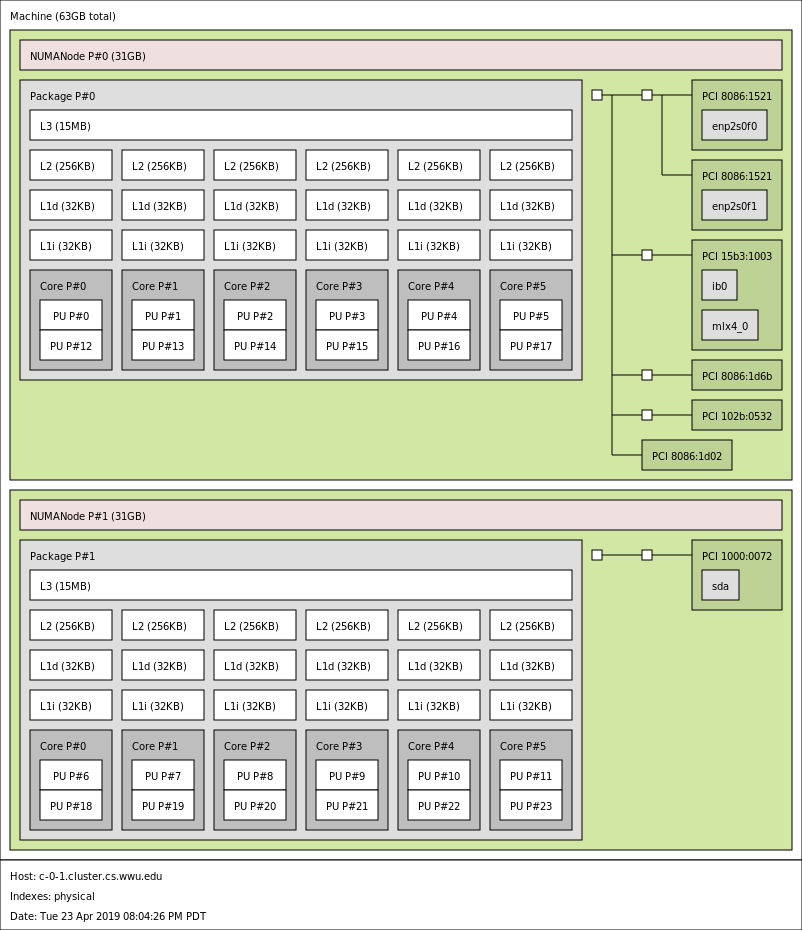
\includegraphics[width=\textwidth]{cluster}
\end{figure}

\begin{itemize}
\item 2 Nodes
\item Node Kind: NUMA
\item 1 Socket per node
\item Cores  
  \begin{itemize}
  \item Cores per socket: 6
    \begin{itemize}
    \item Processing units per core: 2
    \end{itemize}
  \item L3 cache
    \begin{itemize}
    \item Distribution: shared across socket
    \item Size: 15MB
    \end{itemize}
  \item L2 cache
    \begin{itemize}
    \item Distribution: per core
    \item Size: 256KB
    \end{itemize}
  \item L1-data cache
    \begin{itemize}
    \item Distribution: per core
    \item Size: 32KB
    \end{itemize}
  \item L1-instruction cache
    \begin{itemize}
    \item Distribution: per core
    \item Size: 32KB
    \end{itemize}
  \end{itemize}
\end{itemize}

\section {Thread Affinity}

\paragraph {The first program which was ran was designed to spawn 12 threads (one thread per core), and for each thread,
perform groups of computations, sequentially, on unique partitions of large amounts of data. The source code used follows.}

\subsection{Open MP Source code used}

\begin{lstlisting}[language=C]
  #include <stdio.h>
  #include <stdlib.h>
  #include <omp.h>
  int main(int argc, char **argv){
    //Change the following 2 variables to change input parameter size
    int nlocal = atol(argv[1]);//100000000;
    int nsteps = atol(argv[2]);
    // Allocating memory
    double *in = (double*) malloc( (nlocal+2) * sizeof(double));
    double *out = (double*) malloc(nlocal * sizeof(double));
    for (int i=0; i<nlocal+2; i++)
    in[i] = 1.0;
    for (int i=0; i<nlocal; i++)
    out[i] = 0.0;
    double start_time, end_time;
    for (int step=0; step < nsteps; step++) {
      start_time = omp_get_wtime();
      #pragma omp parallel for schedule(static)
      for (int i=0; i < nlocal; i++) {
        out[i] = ( in[i]+in[i+1]+in[i+2] )/3.;
      }
      #pragma omp parallel for schedule(static)
      for (int i=0; i < nlocal; i++){
        in[i+1] = out[i];
      }
      in[0] = 0;
      in[nlocal+1] = 1;
    }
    end_time = omp_get_wtime();
    printf("%lf\n", end_time - start_time);
  }

\end{lstlisting}

\subsection{Results}

\paragraph{The thread affinity program was ran 5 times consecutively. Each benchmark was recorded in seconds, and an average, minimum, and maximum amount were taken for each of them.}

\begin{figure}[h]
\caption{Thread affinity times}
\centering
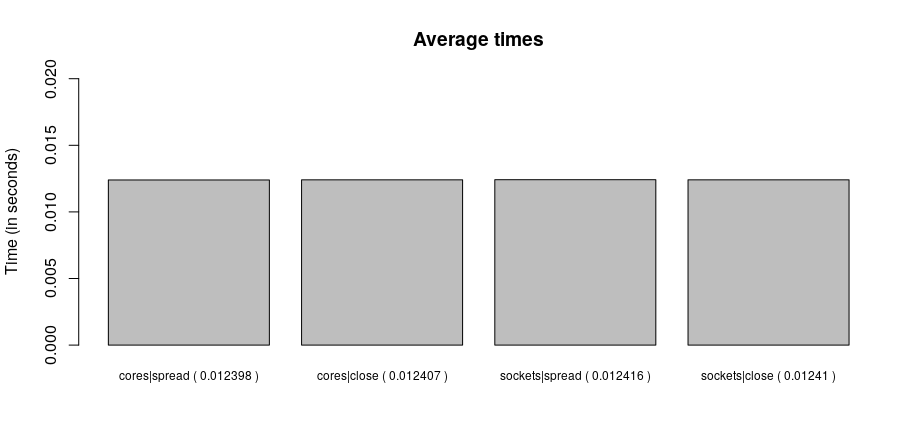
\includegraphics[width=\textwidth]{times_average}
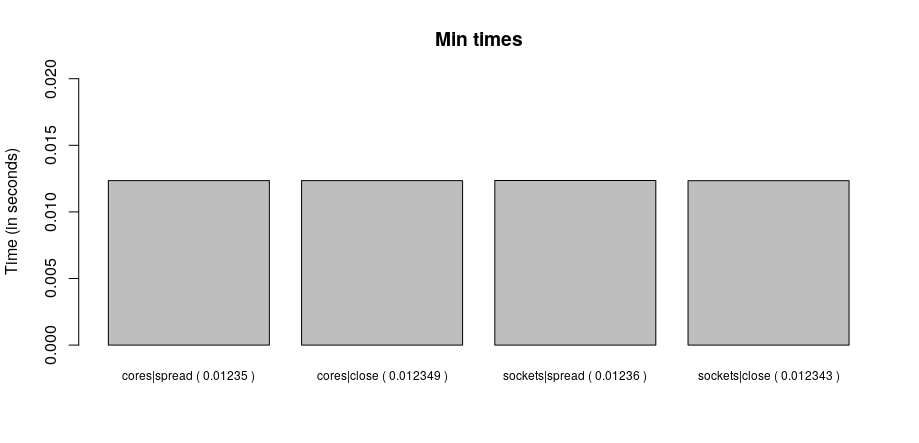
\includegraphics[width=\textwidth]{times_min}
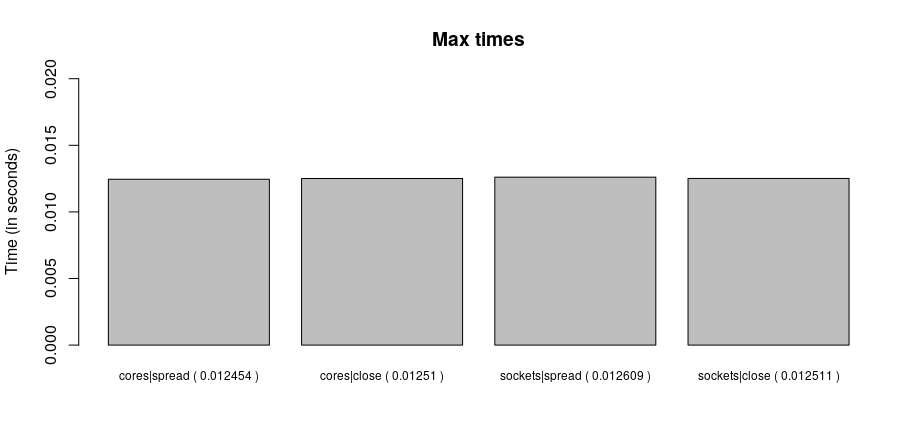
\includegraphics[width=\textwidth]{times_max}
\end{figure}

\paragraph{We used the 4 standard execution profiles provided by OpenMP, which are:}

\begin{itemize}
\item cores spread
  \begin{itemize}
    \item Average time: 0.012390 seconds
    \item Description:

      The idea behind this profile is to spread the amount of threads we allocate throughout multiple cores.
      This allows for us to take advantage of multiple caches, which implies that we have potentially up to 8192 cached elements,
      assuming that, for each core, the respective matrix being iterated over has address values which map into the physical
      page table in such a manner that there is no conflict.
    \end{itemize}
  \item cores close
    \begin{itemize}
    \item Average time: 0.012407 seconds
    \item Description:

      The average listed here is slightly slower, but the difference is essentially negligable. The "close" binding method is designed to cluster threads closer to the same core. The potential for cache thrashing due to multiple threads contesting similar regions of memory is higher in this sense. That said, assuming the implementation associates thread groups contiguously, this is less of an issue, given that other threads are less likely to have conflicting memory regions.
    \end{itemize}
  \item sockets spread
    \begin{itemize}
    \item Average time: 0.012416 seconds
    \item Description:

      This is interesting, because it's more or less around the same amount of time as the previous two. That said, it also makes sense, considering that the memory accesses essentially have a one to one mapping with the thread the group of indices have been accounted for; we don't have iterations which are reaching out in order to fetch data that lies 300000 words away from the current offset that's represented for a given iteration; because of this, we're less likely to have to deal with cross socket memory accesses, which incur significant latency overhead.
    \end{itemize}

  \item sockets close
    \begin{itemize}
    \item Average time: 0.01241 seconds
    \item Description:
      In this profile, we're constraining the 12 threads into one socket, but whether or not the threads are spread throughout different cores (likely) is dependent on the implementation; the specification itself insinuates this [1, pg. 605]
    \end{itemize}
\end{itemize}


\subsection{Conclusion}

\paragraph{It seems logical that the cores spread execution profile would run the fastest: we're using only one thread per core, and despite the NUMA architecture playing a pivotal role in memory access latency, the L1 caches themselves are also per-core, so any reaches out to main memory are few and far between. Furthermore, the way stride of the data for each thread is mapped reduces the need for out of socket memory reads/writes. Of course, it's worth while to consider factors such as how the NUMA architecture searches other out of socket L3 caches if the data it's searching for hasn't been found in its own L3 cache.}


\section{Matrix Multiply}

\section{References}

\begin {enumerate}
\item The OpenMP Application Programming Interface, Version 5.0, The OpenMP Architectural Review Board, November 2018,
  https://www.openmp.org/wp-content/uploads/OpenMP-API-Specification-5.0.pdf
\end{enumerate}

\end{document}